% !TeX spellcheck = de_DE

\newcommand{\tikzInfoVis}{
	\begin{tikzpicture}[
				align = center,
				repr/.style = {
					draw,
					rectangle,
					minimum width = 2cm,
					minimum height = 1cm,
				}
			]
		\node [repr] (rawData) {Rohdaten};
		\node [repr, right = 1.5 of rawData] (dataTables) {Daten-\\tabellen};
		\node [repr, right = 1.5 of dataTables] (visualStructures) {Visuelle\\Strukturen};
		\node [repr, right = 1.5 of visualStructures] (views) {View};
		\node [right = 1 of views] (human) {Mensch};
		\node [right = 1 of human] (task) {Aufgabe};

		\draw [->] (rawData) to node[below, yshift = -0.8cm](dataTransformation){Daten-\\transformation} (dataTables);
		\draw [->] (dataTables) to node[below, yshift = -0.8cm](visualMapping){Visuelle\\Abbildung} (visualStructures);
		\draw [->] (visualStructures) to node[below, yshift = -0.8cm](viewTransformation){View\\Transformation} (views);


		\path (dataTables.south) to coordinate(dataTablesNeedleA) (dataTables.south west);
		\coordinate [below left = 0.5 of dataTables, yshift = 0.15cm] (dataTablesNeedleB);
		\path (dataTables.west) to coordinate(dataTablesNeedleC) (dataTables.south west);

		\path (visualStructures.south) to coordinate(visualStructuresNeedleA) (visualStructures.south west);
		\coordinate [below left = 0.5 of visualStructures, yshift = 0.15cm] (visualStructuresNeedleB);
		\path (visualStructures.west) to coordinate(visualStructuresNeedleC) (visualStructures.south west);

		\path (views.south) to coordinate(viewsNeedleA) (views.south west);
		\coordinate [below left = 0.5 of views, yshift = 0.15cm] (viewsNeedleB);
		\path (views.west) to coordinate(viewsNeedleC) (views.south west);

		\draw [->] (dataTablesNeedleA) |- (dataTablesNeedleB) |- (dataTablesNeedleC);
		\draw [->] (visualStructuresNeedleA) |- (visualStructuresNeedleB) |- (visualStructuresNeedleC);
		\draw [->] (viewsNeedleA) |- (viewsNeedleB) |- (viewsNeedleC);

		\coordinate [below = 2.25 of human] (needle);

		\draw [->] (human) -- (needle) -| (dataTransformation);
		\draw [->] (human) -- (needle) -| (visualMapping);
		\draw [->] (human) -- (needle) -| (viewTransformation);

		\draw [dotted] (task) -- (human);
	\end{tikzpicture}
}

\chapter{Einleitung}
	In dieser Zusammenfassung werden zwei Themen behandelt: Informationsvisualisierung und Visual Analytics. Dabei sollen die Frage beantwortet werden, wie verschiedene Daten \emph{gut} visualisiert werden können und wie Visualisierung die Analyse unterstützen können. Viele Ideen der folgenden Kapitel und grundlegender Techniken bauen dabei auf dem Verständnis grundlegender Prozesse des Gehirns ab. Denn: Eine Visualisierung soll dem Gehirn des*der Nutzer*in Arbeit abnehmen. Dabei sollen für jede Visualisierung die folgenden drei Fragen beantwortet werden:
	\begin{itemize}
		\item Was wird wie dargestellt?: Formale Beschreibung einer Visualisierung.
		\item Was ist gut und (möglichst) ohne Anstrengung sichtbar?: Prinzipien der Wahrnehmung kennen und anwenden.
		\item Was hilft dem*der Nutzer*in bei der Aufgabe?: Beschreibung und Wahrnehmungsprinzipien im Kontext einer Aufgabe bewerten.
	\end{itemize}
	Ein relevantes, bisher noch nicht erwähntes, Wort in den obigen Fragen ist die \emph{Aufgabe}. Zu Beginn jeder Visualisierung muss zunächst die \emph{Aufgabe} der Visualisierung identifiziert werden. Dies sind oftmals Entscheidungen, die (objektiv) durch Daten und Informationen getroffen werden (sollten). Dies ist in \autoref{fig:aufgabe} dargestellt. In der Praxis werden jedoch häufig einfach Visualisierungkataloge (große Datenbanken mit Visualisierungstechniken) nach einer "schönen" Visualisierung durchsucht. Dadurch wird das Dasein der Visualisierung als Werkzeug jedoch zu dem Zweck gemacht, \dh die Visualisierung wird ein Selbstzweck. Dies sollte eigentlich nie der Fall sein!

	Oft die Aussage getroffen, dass "ein Bild mehr sagt als tausend Worte." Im Allgemeinen sollte allerdings eher gesagt werden, dass ein Bild etwas \emph{anderes} als tausend Worte sagt: Sprachliche Artefakte (wozu auch Zahlen gehören), werden von dem Gehirn \emph{bewusst} und verarbeitet und oftmals in eine zeitliche Reihenfolge gebracht. Eine Visualisierung der selben Daten hingegen ist ein bildliches Artefakt und erlaubt eine \emph{unbewusste} Verarbeitung, bei der die Informationen im Raum strukturiert werden. Dadurch können komplexe Zusammenhänge sehr schnell vermittelt und erfasst werden.

	\begin{figure}
		\centering
		\begin{tikzpicture}[->, every node/.style = { draw, rectangle, minimum width = 3cm, minimum height = 0.75cm }]
			\node (daten) {Daten};
			\node [right = 1 of daten] (vis) {Visualisierung};
			\node [right = 1 of vis] (wissen) {Wissen};
			\node [right = 1 of wissen] (entscheidung) {Entscheidung};

			\draw (daten) -- (vis);
			\draw (vis) -- (wissen);
			\draw (wissen) -- (entscheidung);
		\end{tikzpicture}
		\caption[Von Daten zu Entscheidungen]{Eine Visualisierung dient immer der Erfüllung einer Aufgabe und soll zu einem Erkenntnisgewinn führen. Oftmals steht am Ende davon eine Entscheidung, die objektiv durch Daten getroffen werden soll. Bei der Erstellung einer Visualisierung sollte dieser Prozess also rückwärts durchgeführt werden, \dh ausgehend von der Frage, welche Entscheidung getroffen werden soll.}
		\label{fig:aufgabe}
	\end{figure}

	\section{Anwendungen von Visualisierungen}
		Die Anwendung einer Visualisierung, lässt sich in zwei Kategorien einteilen: \emph{Erfassen} und \emph{Produzieren} von Informationen, wobei erstere durch Informationsvisualisierung und letztere durch Visual Analytics "bearbeitet" werden.

		Innerhalb der Informationsvisualisierung werden die folgenden Gruppen unterschieden:
		\begin{itemize}
			\item \eqmakebox[ivAufgaben][l]{\emph{Explain:}} Es sollen bekannte Informationen an andere vermittelt werden (möglicherweise, aber nicht immer, interaktiv).
			\item \eqmakebox[ivAufgaben][l]{\emph{Explore:}} Es sollen neue Information auf Basis von Daten gefunden oder unsichere Informationen bestätigt werden (üblicherweise sehr interaktiv; das Ziel ist nicht immer bekannt).
			\item \eqmakebox[ivAufgaben][l]{\emph{Enjoy:}}   Zwanglose und durch Neugier getriebene Begegnung mit den Daten; dabei ist die Aufgabe selten bekannt.
		\end{itemize}
		Von diesen drei Arten der Informationsvisualisierung werden in dieser Zusammenfassung vor allem die ersten beiden behandelt.

		Innerhalb der Visual Analytics werden die folgenden Gruppen unterschieden:
		\begin{itemize}
			\item \eqmakebox[vaAufgaben][l]{\emph{Annotate}}
			\item \eqmakebox[vaAufgaben][l]{\emph{Record}}
			\item \eqmakebox[vaAufgaben][l]{\emph{Derive}}
		\end{itemize}
	% end

	\section{Identifizierung der Visualisierungsaufgabe}
		Bei der Identifizierung der Aufgabe sollte auch mit einbezogen werden,
		\begin{itemize}
			\item welche Informationen als bekannt vorausgesetzt werden,
			\item welche Informationen gesucht werden, und
			\item was mit den neuen Informationen gemacht wird oder gemacht werden soll.
		\end{itemize}
		Das Design der Visualisierung bestimmt damit essentiell, wie gut mit der Visualisierung gearbeitet werden kann durch Wiedererkennung bekannter Informationen und Erkennung neuer Informationen. Die erste Regel ist dabei, wie bereits erwähnt, das die Visualisierung ein Werkzeug und kein Selbstzweck ist. Das lässt sich wie folgt zusammenfassen:
		\begin{center}
			Have something to tell or something to ask!
		\end{center}
	% end

	\section{Negativbeispiele} % 1.47, 1.48, 1.49, 1.50, 1.51, 1.52, 1.53, 1.54, 1.55, 1.56, 1.57, 1.58, 1.59
		\todo{Content}
	% end
% end

\chapter{Der Informationsvisualisierungsprozess}
	\label{c:visualisierungsprozess}

	Der \emph{Informationsvisualisierungsprozess}, dargestellt in \autoref{fig:visualisierungsprozess}, wurde von Card et al. als Referenzmodell entworfen, um die Erstellung einer Visualisierung zu strukturieren. Dabei wird zwischen den Repräsentationen (\emph{Rohdaten}, \emph{Datentabellen}, \emph{Visuelle Strukturen} und \emph{Views}) unterschieden. Der Übergang zwischen den Strukturen wird durch die \emph{Datentransformation}, die \emph{Visuelle Abbildung} und die \emph{View Transformation} beschrieben. Eine weitere Zentrale Komponente ist der*die Nutzer*in (\emph{Mensch}), welche*r die einzelnen Schritte modifiziert. Dadurch wird das Modell zu einem Kreislauf der Visualisierung. In diesem Kapitel wird jeder Schritt separat behandelt, beginnend mit der Datentransformation (\autoref{sec:dataTransformation}) über die visuelle Abbildung (\autoref{sec:visualMapping}) bis zur Interaktion (\autoref{sec:interaktion}). Im folgenden wird eine kurze Übersicht über die Transformationsschritte gegebene:
	\begin{itemize}
		\item \eqmakebox[infoVisProzess][l]{\emph{Datentransformation:}} Der der \emph{Datentransformation} werden die \emph{Rohdaten} in \emph{Datentabellen} umgewandelt. Diese können dann in den nächsten Schritten einfacher als die Rohdaten verarbeitet werden, da diese häufig ungeordnet und unstrukturiert vorliegen.
		\item \eqmakebox[infoVisProzess][l]{\emph{Visuelle Abbildung:}}  Bei der \emph{visuellen Abbildung} findet der Hauptteil der Visualisierung statt. Dabei werden einzelne Datenvariablen auf visuelle Attribute (\bspw die Position) abgebildet, was die \emph{visuellen Strukturen}.
		\item \eqmakebox[infoVisProzess][l]{\emph{Datentransformation:}} Abschließend werden in der \emph{View Transformationen} die tatsächlichen Datenwerte auf die Variablenwerte der visuellen Struktur abgebildet, woraus sich die tatsächliche Visualisierung, die \emph{View}, ergibt.
	\end{itemize}
	Die Unterscheidung zwischen der visuellen Abbildung und der View Transformation ist, dass ersteres beschreibt, \emph{dass} eine Datenvariable auf eine visuelle Variable abgebildet wird, und letzteres beschreibt, \emph{welcher} konkrete Datenpunkt auf welchen konkreten Wert abgebildet wird.

	Der letzte Schritt im Informationsvisualisierungsprozess ist die Interaktion, welche durch die zurückgeführten Pfeile in \autoref{fig:visualisierungsprozess} dargestellt wird. Dies ist die technische Möglichkeit, die einzelnen Schritte zu verändern und anzupassen. Es soll dem*der Nutzer*in dabei möglich sein, einzelne Komponenten anzupassen, ohne auf eine neue Visualisierung des*der Designer*in zu warten. Für den*die Designer*in kann dadurch zu teilen das Problem gelöst werden, dass eventuell die genaue Aufgabe noch nicht bekannt ist.

	\begin{figure}
		\centering
		\tikzInfoVis
		\caption[Informationsvisualisierungsprozess]{Der Informationsvisualisierungsprozess nach Card et al.}
		\label{fig:visualisierungsprozess}
	\end{figure}

	\section{Die Datentransformation}
		\label{sec:dataTransformation}

		Bei der Datentransformation werden die Rohdaten in Datentabellen umgewandelt, welche in den folgenden Schritten einfacher zu verarbeiten sind. Außerdem können eine Reihe an Vorverarbeitungstechniken (\bspw Datenbereinigung) angewandt werden. Dieser Abschnitt führt zunächst in die grundlegenden Datentypen und -strukturen sowie anschließend verschiedene Techniken der Vorverarbeitung ein.

		\subsection{Datentypen und Datenstrukturen}
			Zur Diskussion und Abbildung von Daten auf visuelle Strukturen ist es zunächst sinnvoll, die verschiedenen auftretenden Datentypen und -strukturen zu betrachten. Die Unterscheidung zwischen einem Typ und einer Struktur wird dabei grundlegend durch die Anzahl der zugeordneten Datenvariablen getroffen: Einfache Datentypen beziehen sich immer auf genau eine Datenvariable während Datenstrukturen Beziehungen zwischen mehreren Datenvariablen (welche meist Eigenschaften von Objekten, auch \emph{Items} genannt, sind) und Datensätzen beschreiben. Eine Visualisierung kann anschließend eine beliebige Kombination aus Datenvariablen, Items und Beziehungen abbilden.

			\subsubsection{Datentypen}
				Grundlegend wird zwischen \emph{nominalen}, \emph{ordinalen} und \emph{quantitativen} Datentypen unterschieden. Bei einem nominalen Datentyp ist dabei zwischen zwei Werten nur \emph{Gleichheit} und \emph{Ungleichheit} definiert. Dies können \zB Personen, Länder, etc. sein. Sind nur nominelle Daten zu visualisieren, kann eine Tabelle hier tatsächlich die beste Wahl sein! Ordinale Datentypen haben zusätzlich zu (Un-) Gleichheit noch eine \emph{Ordnung}, \bspw Schulnoten oder Rangordnungen. Der in Anzahl Operationen "mächtigste" Datentyp sind quantitative Daten, die auch noch \emph{Differenzen} und \emph{Differenzverhältnisse} haben. Ferner wird bei quantitativen Daten zwischen \emph{diskreten} und \emph{kontinuierlichen} Daten. Außerdem gibt es \emph{Intervall-} und \emph{Verhältnisskalen}: Auf ersterer sind Verhältnisse nicht vernünftig berechenbar, da die Skala keinen natürlichen Nullpunkt hat (\bspw Temperatur in \si{\degreeCelsius}). Letztere hat einen natürlichen Nullpunkt, weshalb auch Verhältnisse auf Werten Sinn ergeben (\bspw Temperatur in Kelvin). Des weiteren gibt es \emph{lineare} und \emph{zyklische} Skalen, bei der die Ordnung eine Totalordnung, \bzw eine "künstliche" Ordnung, ist.

				Die unterschiedlichen Datentypen sind in \autoref{fig:datentypen} zusammengefasst. Im Allgemeinen lässt sich also sagen, dass sich Datentypen vor allem durch die auf ihnen ausführbaren Operatoren unterscheiden. Außerdem ist nicht die Repräsentation, sondern die Bedeutung des Datentyps relevant (\bspw sehen Schulnoten aus wie Zahlen, sind aber ordinale Daten).

				\begin{figure}
					\centering
					\begin{tikzpicture}[align = center, class/.style = { draw, rectangle, minimum width = 3cm, minimum height = 0.75cm }]
						\node [class] (datentypen) {\textbf{Datentypen}};

						\node [class, below = 1.5 of datentypen, xshift = -5cm] (nominal) {\textbf{Nominal}};
						\coordinate [below = 0.5 of nominal] (a);
						\node [right = 0.5 of a] (aa) {\eqmakebox[datentypenNominal][l]{(Un-) Gleichheit}};
						\draw (nominal) |- (aa);

						\node [class, below = 1.5 of datentypen] (ordinal) {\textbf{Ordinal}};
						\coordinate [below = 0.5 of ordinal] (b);
						\node [right = 0.5 of b] (ba) {\eqmakebox[datentypenOrdinal][l]{(Un-) Gleichheit}};
						\node [below = 0 of ba] (bb) {\eqmakebox[datentypenOrdinal][l]{Ordnung}};
						\draw (ordinal) |- (ba);
						\draw (ordinal) |- (bb);

						\node [class, below = 1.5 of datentypen, xshift = 5cm] (quantitativ) {\textbf{Quantitativ}};
						\coordinate [below = 0.5 of quantitativ] (c);
						\node [right = 0.5 of c] (ca) {\eqmakebox[datentypenQuantitativ][l]{(Un-) Gleichheit}};
						\node [below = 0 of ca] (cb) {\eqmakebox[datentypenQuantitativ][l]{Ordnung}};
						\node [below = 0 of cb] (cc) {\eqmakebox[datentypenQuantitativ][l]{Differenzen}};
						\node [below = 0 of cc] (cd) {\eqmakebox[datentypenQuantitativ][l]{Differenzverhältnisse}};
						\node [below = 0 of cd] (ce) {\eqmakebox[datentypenQuantitativ][l]{Diskret/Kontinuierlich}};
						\node [below = 0 of ce] (cf) {\eqmakebox[datentypenQuantitativ][l]{Intervall-/Verhältnisskala}};
						\node [below = 0 of cf] (cg) {\eqmakebox[datentypenQuantitativ][l]{Linear/Zyklisch}};
						\draw (quantitativ) |- (ca);
						\draw (quantitativ) |- (cb);
						\draw (quantitativ) |- (cc);
						\draw (quantitativ) |- (cd);
						\draw (quantitativ) |- (ce);
						\draw (quantitativ) |- (cf);
						\draw (quantitativ) |- (cg);

						\path (datentypen) to coordinate(needle) (ordinal);
						\draw (datentypen) -- (needle) -| (nominal);
						\draw (datentypen) -- (ordinal);
						\draw (datentypen) -- (needle) -| (quantitativ);
					\end{tikzpicture}
					\caption{Unterschiedliche Datentypen}
					\label{fig:datentypen}
				\end{figure}
			% end

			\subsubsection{Datenstrukturen}
				Die bisher diskutierten Daten\emph{typen} beziehen sich immer auf genau eine Datenvariable, wohingegen Daten\emph{strukturen} auch Zusammenhänge zwischen Daten abbilden. Dabei sind Datenvariablen oft Eigenschaften von Objekten, die hier \emph{Item} genannt werden.

				Die einfachste Form einer Datenstruktur ist eine Tabelle, die außerdem sehr flexibel ist, weshalb sie im Informationsvisualisierungsprozess (\autoref{fig:visualisierungsprozess}) namensgebend ist. Innerhalb einer Tabelle hat jede Spalte eine von zwei Rollen: Key oder Value. Dabei definieren die Datentype der Keys die eigentliche Datenstruktur und die Values sind von den Keys abhängig. Dabei müssen die Keys eine Zeile eindeutig identifizieren, \dh es darf keine Kombination mehrfach auftreten.

				Hat eine Tabelle keine Keys sondern ausschließlich Attribute, so werden die Items nur technisch Unterschieden (\bspw durch eine Zeilennummer) und die Daten sind "rein" uni-/bi-/multivariat. Dies ist oft der Fall bei Daten, bei denen die Eigenschaften wichtiger sind als die Identifikation oder bei Daten, in denen die Items nicht identifiziert werden dürfen (Anonymisierung).

				Da eine Tabelle sehr flexibel ist, sind die folgenden Datenstrukturen allesamt auf eine Tabelle abbildbar (die Abbildung ist jeweils durch die Angabe der Keys gegeben). Darüber hinausgehend gibt es auch Datenstrukturen, die am besten auf mehrere Tabellen (als relationales Modell) abgebildet werden. Achtung: Zwar ist die Darstellung als Tabelle hier zweckmäßig, jedoch müssen die Daten nicht zwangsweise technisch als Tabelle gespeichert werden!

				\paragraph{Zeitbezogene Daten}
					Zeitbezogene Daten haben mindestens einen Zeitstempel als Key, welcher sowohl relativ als auch absolut sein kann. Die Zeit wird häufig über die Position Achse visualisiert (\zB Corona-Fallzahlen). Die Darstellung zeitbezogener Daten wird intensiv in \autoref{sec:visZeitbasiert} behandelt.
				% end

				\paragraph{Ortsbezogene Daten}
					Bei ortsbezogenen Daten ist mindestens ein Key eine Ortsangabe, die beispielsweise als geographische Position (Längen- und Breitengrad) oder Ortsname realisiert werden kann. Eine beliebte Darstellung ist das Anzeigen auf einer Karte.
				% end

				\paragraph{Bewegungsdaten}
					Bewegungsdaten stellen eine Kombination aus zeit- und ortsbezogenen Daten dar. Auch hierbei gibt es mehrere Varianten, \bspw können Messungen an mehreren, aber individuell festen Orten, durchgeführt werden (\zB Wetterstationen) oder die Messungsorte können sich bewegen (\zB Sportdaten). Eine beliebte Darstellung dieser Daten ist eine Karte, wahlweise als 3D-Darstellung mit der Höhe als Zeit. Dadurch sind schnelle und langsame Bewegungen unterscheidbar und Kreuzungen im Raum entsprechen Treffpunkten.
				% end

				\paragraph{Graphen und Netzwerke}
					Graphen und Netzwerke sind spezielle komplexe Datenstrukturen, wobei die Kanten durch zwei Keys desselben Typs auf eine Tabelle abgebildet werden können (die Values sind dann Eigenschaften der Kante, nicht der Knoten). Die Darstellung solcher Daten wird intensiv in \autoref{sec:visGraphen} behandelt.
				% end

				\paragraph{Bäume und Hierarchien}
					Ein Baum kann als Spezialfall eines Graphs behandelt werden, wobei ein Value-Attribut den Key eines anderen Eintrags enthält, wodurch eine Kindheits-Relation induziert wird. Alternativ wäre eine Darstellung als Kantenliste, analog zu einem allgemeinen Graph, möglich. Im Vergleich zu allgemeinen Graphen gibt es für Bäume viele spezialisierte Visualisierungswerkzeuge, die in \autoref{sec:visGraphen} behandelt werden. Dies geschieht durch die Ausnutzung der Ordnungsrelation, die durch einen Baum definiert wird.
				% end
			% end
		% end

		\subsection{Vorverarbeitung}
			Ein wichtiger Teil der Datentransformation stell die Datenvorverarbeitung dar\footnote{Nach einer Studie von CrowdFlower im Jahr 2016 entfällt \SI{80}{\percent} der Zeit bei der Erstellung einer Visualisierung auf die Datensuche und -vorverarbeitung und nur etwas \SI{20}{\percent} auf die eigentliche Visualisierung.}. Da reale Daten oft "unsauber" sind, müssen diese bereinigt werden, um dem "Garbage In, Garbage Out"-Prinzip zu entgehen. \emph{Unsauber} hat dabei viele Facetten, \zB unvollständige und fehlende Werte, Rauschen, Inkonsistenz, Ausreißer und unglaubwürdiger Werte, und viele mehr. Die Vorverarbeitung umfasst dabei alle notwendigen Transformationen, die nicht von dem*der Nutzer*in durchgeführt werden können oder sollen. Wie immer ist die genaue Abgrenzung jedoch Abhängig von der Aufgabe und dem*der Nutzer*in: Ist das Fehlen von Werten beispielsweise keine wertvolle Information für den*die Nutzer*in, so sollten diese in der Vorverarbeitung von dem*der Entwickler*in bereinigt werden. Ein anderes Beispiel sind Ausreißer oder unplausible Werte: Ist der*die Entwickler*in bei der Interpretation der Daten überfordert, sollte die Verarbeitung als Datentransformation interaktiv durch den*die Nutzer*in durchführbar sein. Der Einfachheit halber wird deshalb im folgenden immer von (Daten-) Vorverarbeitung gesprochen, wobei jeder Schritt auch als interaktive Transformation dargestellt werden könnte.

			Bei der Vorverarbeitung sind insbesondere Metadaten (\zB Attributnamen, Referenzpunkte von Messungen, Einheiten, wichtige Schlüsselwörter) hilfreich. Außerdem werden häufig statistische Methoden wie Ausreißererkennung, Clusteranalyse, Korrelationsanalyse sowie statistische Plots und Histogramme verwendet.

			\subsubsection{Fehlende Werte und Datenbereinigung}
				Um fehlende Werte in den Daten zu korrigieren gibt es einige grundlegende Verfahren:
				\begin{itemize}
					\item \eqmakebox[vorverarbeitungFehlende][l]{\emph{Ignorieren:}} Die fehlenden Werte werden ignoriert und es wird gehofft, dass dies in der Visualisierung nicht tiefgreifend durchschlägt.
					\item \eqmakebox[vorverarbeitungFehlende][l]{\emph{Manuell Einfügen:}} Unter Nutzung von Expert*innenwissen werden die Daten manuell ergänzt. Dies ist zwar präzise, aber sehr zeitaufwendig.
					\item \eqmakebox[vorverarbeitungFehlende][l]{\emph{Eliminieren der Zeile:}} Zeilen mit fehlenden Werten werden entfernt. Dies ist die häufigste Methode, jedoch fehlt bei vielen Datensätzen in jeder Zeile mindestens ein Wert.
					\item \eqmakebox[vorverarbeitungFehlende][l]{\emph{Globale Konstante:}} Anstelle der fehlenden Werte wird eine globale Konstante, \zB \(-1\), eingesetzt. Dies verändert allerdings die Datenverteilung, was Probleme bei statistischen Analysen hervorrufen kann.
					\item \eqmakebox[vorverarbeitungFehlende][l]{\emph{Mittelwert:}} Die Werte werden durch den Mittelwert ersetzt. Dies ist gut für eine globale Statistik, die individuellen Abweichungen können allerdings groß sein.
					\item \eqmakebox[vorverarbeitungFehlende][l]{\emph{Wert basierenden auf Ähnlichkeit:}} Ersetzung der Werte durch Annahme, welche anderen Zeilen "ähnlich" sind.
				\end{itemize}
				Die konkrete Wahl einer dieser Methoden hängt dabei -- wie üblich -- stark von dem vorliegenden Problem ab, \zB des Typs und der Semantik der Daten, der Menge der fehlenden Werte und der Expertise des*der Anwenders*Anwenderin. Im Allgemeinen sollte immer versucht werden, den Grund für das Fehlen zu ermitteln. Außerdem muss bei einem Ersetzen der fehlenden Werte gespeichert werden, dass es sich um Ersatzwerte handelt!

				Im falle von fehlerhaften Werten, die häufig durch Menschen selbst verursacht werden, können ähnliche Methoden eingesetzt werden, allerdings sind diese sehr viel schwer zu detektieren.
			% end

			\subsubsection{Ausreißer (-detektion)}
				\emph{Ausreißer} sind Datenpunkte, die außerhalb des normalen Wertebereichs einer Datenvariable liegen. \emph{Starke} Ausreißer sind solche, die für Expert*innen ungewöhnlich und interessant sind. Dabei ist es nicht immer einfach zu entscheiden, was ein interessanter -- aber plausibler -- Ausreißer und was ein Fehler ist. Zur Detektion von Ausreißern werden deshalb häufig statistische Verfahren herangezogen. Eine einfache Methode ist die Annahme einer Normalverteilung und Ausschluss aller Werte, die um mehr als zwei Standardabweichungen vom Mittelwert abweichen. Das offensichtliche Problem dieser Annahme ist, dass sie häufig nicht gilt (\bspw da die Daten von mehreren Normalverteilungen stammen; dies kann durch Clustering detektiert werden, was später behandelt wird \todo{ref clustering}). Allerdings können, wie bereits erwähnt, Ausreißer auch plausibel und somit keine Datenfehler sein (ein Beispiel hierfür ist die Temperatur auf der Zugspitze, die plausibel einen Ausreißer im Vergleich zu meeresspiegelnahen Messstation darstellt).
			% end

			\subsubsection{Normalisierung und Skalierung}
				Oftmals würde ein einfaches Anzeigen der Daten dazu führen, dass viele der Datenpunkte an einem Ende der Skala "kleben." Hier kann eine Skalierung der Daten abhelfen, indem die Daten auf irgendeine Weise gestreckt/gestaucht werden. Dabei werden die Daten auf ein "normales" Intervall, \zB \([0, 1]\) oder \([-1, 1]\), abgebildet. Gängige Methoden sind:
				\begin{itemize}
					\item Min-Max-Normalisierung
						\begin{itemize}
							\item Linear
							\item Logarithmisch
							\item Wurzel
							\item Quadratisch
							\item Exponentiell
						\end{itemize}
					\item Weitere datenspezifische Normalisierungen (\bspw nach der Objektform)
					\item z-Score
					\item Quantil-Normalisierung
				\end{itemize}
				Bei der Min-Max-Normalisierung wird das Minimum \(\ell\) und das Maximum \(u\) der Daten verwendet, um die restlichen Daten zu skalieren. Zur Abbildung auf das Intervall \( [0, 1] \) gibt es \zB die folgenden Methoden\footnote{Zur Interpretation der logarithmischen Normalisierung kann es hilfreich sein, diese etwas umzuformen: \( (\log x - \log \ell) / (\log u - \log \ell) = \log(x/\ell) / \log(u/\ell) = \log_{u/\ell}(x/\ell) = \log_{u/\ell} x + \const_x \)}:
				\begin{align}
					f_\text{Linear}(x) &= \frac{x - \ell}{u - \ell} &
					f_\text{Log}(x) &= \frac{\log x - \log \ell}{\log u - \log \ell} &
					f_\text{Quad}(x) &= \bigl( f_\text{Linear}(x) \bigr)^2 &
					f_\text{Wurzel} &= \sqrt{f_\text{Linear}(x)}
				\end{align}
				Für eine Normalisierung in den Bereich \( [-1, 1] \), was für negative, "bipolare", Werte sinnvoll ist, kann \zB wieder eine Min-Max-Normalisierung
				\begin{align}
					\hat{f}_\text{Linear}(x) &= 2 f_\text{Linear})(x) - 1
				\end{align}
				eingesetzt werden. Dabei kann es hilfreich sein, \(\ell\) und \(u\) als die absoluten Minima und Maxima zu definieren, \dh
				\begin{align}
					\ell' &= -\max\{ \lvert \ell \rvert, u \} &
					u' &= \max\{ \lvert \ell \rvert, u \},
				\end{align}
				um sicherzustellen, dass \( \hat{f}_\text{Linear}(0) = 0 \) gilt (dies kann sonst zu einer Verzerrung führen, \bspw bei Temperaturen).

				\paragraph{Lokale und Globale Skalierung}
					Gibt es mehrere Datensätze mit unterschiedlichen Minima/Maxima (\zB Temperaturverlauf in mehreren Städten), so muss entschieden werden, welche Minima/Maxima verwendet werden. Dabei wird zwischen \emph{lokaler} und \emph{globaler} Normalisierung unterschieden: Bei der lokalen Normalisierung werden die Minima/Maxima jeden Datensatz bestimmt und angewendet, bei der globalen Normalisierung wird das Minimum/Maximum über alle Datensätze hinweg verwendet.

					Dabei gilt, wie so oft, dass die konkrete Wahl auch von dem konkreten Problem abhängt. Während bei einer lokalen Normalisierung die Wertverläufe gut verglichen werden können (\dh wann unterschiedliche Reihen \zB ihr Maximum erreichen), so können dabei die Werte nicht mehr direkt verglichen werden. Komplementär dazu können die Werte bei einer globalen Normalisierung gut verglichen werden, bei großen Unterschieden ist ein Verlaufsvergleich jedoch sehr schwer.
				% end
			% end

			\subsubsection{Diskretisierung}
				Werden kontinuierliche Daten verarbeitet, so ist es häufig nötig, diese zu diskretisieren, \dh diskrete Teilmengen als Approximation zu finden. Der Hauptgrund dafür ist, dass ein digitales System nicht mit "echt"-kontinuierlichen Daten umgehen kann, da sie inhärent diskret sind. Die üblichste Diskretisierungsdimension ist dabei die Zeit, bei der ein beliebiger Punkt \( t_k = k \Delta_t \) für einen Zeitindex \(k\) mit vorgeschriebener Schrittweite \(\Delta_t\) diskretisiert wird. Bei der Diskretisierung gehen allerdings Informationen verloren, was eventuell problematisch werden kann (vgl. Nyquist-Shannon-Abtasttheorem).
			% end

			\subsubsection{Sampling, Segmentierung und Untermengen}
				Um die Datenmenge zu reduzieren, gibt es verschiedene Ansätze. Eine davon ist \emph{Sampling}, wobei zufällige Stichproben aus den Daten gezogen werden, um die Datenpunkte in der Visualisierung zu reduzieren. Je nach Wahl der Verteilungsfunktion kann sich dadurch allerdings eine Verzerrung in den Daten und einiger statistischer Eigenschaften ergeben. Andere, nicht-zufalls-basierte, Methoden sind \emph{Segmentierung} und die Wahl von \emph{Untermengen}. Bei der Segmentierung werden die Daten in zusammenhängende Abschnitte/Regionen eingeteilt und einer Kategorie zugeordnet. Dies ist allerdings nicht immer eindeutig möglich. Die Wahl von Untermengen kann \bspw auf Basis von Filtern und anderen Einschränkungen erfolgen.
			% end

			\subsubsection{Datenintegration}
				Bei der \emph{Datenintegration} werden verschiedene Datenquellen zu einer einzigen Datenquelle vereint, was eventuell die Angleichung von Schemata und ähnlichem erfordert. Beispielsweise müssen bei der Integration imperialistischer und metrischer Quellen die Einheiten angepasst werden.
			% end
		% end
	% end

	\section{Die Visuelle Abbildung}
		\label{sec:visualMapping}

		In diesem Abschnitt wird die visuelle Abbildung, der dritte Schritt im Visualisierungsprozess (\autoref{fig:visualisierungsprozess}) genauer behandelt. Dabei ist die Abgrenzung zum vierten Schritt, der View Transformation, nicht immer scharf gezogen, da die Schritte eng zusammenhängen. In der Regel wird in der visuellen Abbildung eine Datenvariable auf eine visuelle Struktur abgebildet. Dies muss aber nicht immer exakt sein, \dh eine Variable kann auch auf mehrere Strukturen oder mehrere Variablen können auf die gleiche Struktur abgebildet werden (\bspw wird in einer Scatterplot-Matrix sowohl ein Datenwert als auch eine Dimension auf die Position abgebildet). Im Folgenden werden einige visuelle Strukturen ("Marks" und "Channels") eingeführt und ihre typische Anwendung beschrieben.

		Eine visuelle Abbildung muss immer die folgenden Dinge beinhalten: Titel, Skala und Achsenbeschriftungen (gegebenenfalls mit Einheit), Datenquelle, Legende und den Grafikkörper selbst. Außerdem sollte üblicherweise eine Bildunterschrift mit angegeben werden, siehe dazu \autoref{subsec:caption}.

		\subsection{Beispiele}
			\todo{Die Visuelle Abbildung: Beispiele; 2.3, 2.4, 2.5, 2.6; 2.7, 2.8, 2.9; 2.10, 2.11, 2.12}
		% end

		\subsection{Visuelle Strukturen}
			In diesem Abschnitt werden eine visuelle Strukturen -- auch \emph{Marks} und \emph{Channels} genannt -- eingeführt und ihre übliche Einsetzung beschrieben. Dabei beginnt jede Visualisierung grundlegend mit einem leeren Blatt, dem die visuellen Strukturen hinzugefügt werden.

			Der \emph{Raum}, \dh die Position auf der Abbildung, ist die bei weitem wichtigste und vielseitigste Struktur. Sofern nicht anders angegeben beziehen sich die Positionen immer auf zwei unabhängige\footnote{Die Wortwahl \emph{unabhängig} bezieht sich hier nur darauf, dass die Variablen selbst, nicht zwangsweise die Werte, unabhängig sind.} Variablen (\(x\) und \(y\)). Die Position ist dabei auch die einzige Struktur, die unabhängig von der Aufgabe und dem Datentyp verwendet werden kann und -- ebenfalls als einzige Struktur -- verwendet werden muss. Daher ist die Belegung der visuellen Raumvariablen die erste und wichtigste Designentscheidung. Innerhalb des Raumes werden anschließend weitere visuelle Strukturen platziert, die in Marks und Channels eingeteilt sind: \emph{Marks} sind geometrische Elemente, aus denen die Visualisierung zusammengesetzt sind, während \emph{Channels} Eigenschaften der Markierungen/Marks sind.

			Die visuelle Abbildungen besteht abschließend aus einer Zuordnung von Datenvariablen und Merkmalen auf Marks und Channels, siehe \autoref{fig:marksChannels}.

			\begin{figure}
				\centering
				\begin{tikzpicture}[->, blob/.style = { draw, rectangle, minimum height = 0.75cm, minimum width = 2cm }]
					\node [blob, label = above:Datenobjekt] (item) {Item};
					\node [blob, right = 4 of item, label = above:Merkmal] (value) {Wert};
					\node [blob, below = 2 of item, label = below:Visuelles Objekt] (mark) {Mark};
					\node [blob, right = 4 of mark, label = below:Visuelles Merkmal] (channel) {Channel};

					\draw (item) to node[above]{hat Merkmal} (value);
					\draw (item) to node[left]{Visuelle Abbildung} (mark);
					\draw (value) to node[right]{Visuelle Abbildung} (channel);
					\draw (mark) to node[below]{hat Merkmal} (channel);
				\end{tikzpicture}
				\caption{Beziehung zwischen Items, Werte, visuellen Channels und Marks}
				\label{fig:marksChannels}
			\end{figure}

			\subsubsection{Marks}
				\emph{Marks} sind die eigentlichen Strukturelemente, die auf der Visualisierung abgebildet werden, die häufig jeweils ein Item oder eine Relation repräsentieren. Die üblichsten sind dabei \emph{Punkte}, \emph{Linien}, \emph{Flächen} und \emph{Text} wobei letzterer nur sehr sparsam und am besten gar nicht eingesetzt werden sollte. Zur Auswahl eines Marks sollten mehrere Aspekte in Betracht gezogen werden, insbesondere die Daten, die repräsentiert werden sollen (einzelne Items, Item-Paare, Teilmengen von Items, ein Attribut, etc.). Zum Verständnis der Visualisierung kann es hilfreich sein, wenn eine eingängige Metapher zwischen den repräsentierten Daten und der Visualisierung besteht (\zB Darstellung eines Volumens durch eine Fläche). Dabei stellen Linien häufig dar, dass ein Änderung kontinuierlich verläuft, während Punktmengen und ähnliches andeuten, dass eine Änderung diskret ist. Des weiteren sollte bei der Auswahl der Marks darauf geachtet werden, dass die genutzten Marks die benötigten Channels (siehe nächster Abschnitt) unterstützen.

				Eine Ambiguität zwischen den obigen Marks ist die Unterscheidung zwischen einem Punkt und einer Fläche: Wann ist ein Punkt "so groß", dass er eigentlich eine Fläche ist? Dies kann dadurch aufgelöst werden, dass ein Punkt allgemein eine Markierung bezeichnet, die etwas 0-Dimensionales darstellt, \dh auch ein großer Punkt markiert ausschließlich einen Punkt, indem der Bezug zum Hintergrund verschieden ist.
			% end

			\subsubsection{Channels}
				\label{subsubsec:channels}

				\emph{Channels} sind die visuellen Eigenschaften von Marks, \dh diese können zusätzlich als Unterscheidungs- und Identifikationsmerkmal eingesetzt werden. Dabei unterscheiden sich die anwendbaren Channels nach den eingesetzten Marks. Eine Übersicht über die üblichsten Channels ist in \autoref{fig:channels} zu finden. In diesem Abschnitt werden diese üblichen Channels sowie einige nicht häufig anzutreffende Channels vorgestellt. Ebenfalls wird auf die Rolle der Elemente im Designprozess eingegangen, wobei der Grund für diese Rolle in \autoref{sec:wahrnehmung} behandelt wird. Eine Übersicht über die Eignung der gängigsten Channels für verschiedene Datentypen und Aufgaben ist in \autoref{tab:channelsDatentypen} \bzw \autoref{tab:channelsAufgaben} gegeben.

				Im allgemeinen sollten nicht zu viele Channels verwendet werden, da die Abbildung dadurch chaotisch wird. Im konkreten Fall hängt die genaue Anzahl natürlich immer von der Aufgabe ab. Für Explain- und Explore-Aufgaben sollten generell eher weniger Channels verwendet werden, damit die Visualisierung verständlich bleibt. Außerdem sollte bei "Explore" vermieden werden, dass dominante Channels die Wahrnehmung von Mustern in anderen Channels verhindern. Bei "Enjoy" hingegen ist absolute Freiheit gegeben.

				\begin{table}
					\centering
					\begin{tabular}{l|l|l}
						\toprule
						\textbf{Punkt} & \textbf{Linie}                       & \textbf{Flächen}                  \\ \midrule
						Position       & Position                             & Position                          \\
						Farbe          & Farbe                                & Farbe                             \\
						Helligkeit     & Helligkeit                           & Helligkeit                        \\
						Form           & Breite                               & Kanteneigenschaften (siehe Linie) \\
						Orientierung   & Stil (Gestrichelt, Gepunktet, \dots) & Tiefe                             \\
						Größe          & Größe/Länge                          & Größe/Fläche                      \\
						Textur         & Dynamik                              & Textur                            \\ \bottomrule
					\end{tabular}
					\caption{Übliche Channels}
					\label{fig:channels}
				\end{table}

				\begin{table}
					\centering
					\begin{tabular}{c|ccccc}
						\toprule
						                       & \textbf{Nominal} & \textbf{Ordinal} & \textbf{Quantitativ} & \textbf{Räumlich} & \textbf{Zeitlich} \\ \midrule
						  \textbf{Position}    &      \(+\)       &      \(+\)       &        \(+\)         &       \(+\)       &       \(+\)       \\
						    \textbf{Länge}     &      \(-\)       &      \(+\)       &        \(+\)         &       \(?\)       &       \(?\)       \\
						    \textbf{Größe}     &      \(-\)       &      \(+\)       &      \(\circ\)       &       \(-\)       &       \(-\)       \\
						\textbf{Farbsättigung} &      \(-\)       &      \(+\)       &      \(\circ\)       &       \(-\)       &       \(-\)       \\
						   \textbf{Textur}     &      \(+\)       &      \(+\)       &        \(-\)         &       \(-\)       &       \(-\)       \\
						   \textbf{Farbton}    &      \(+\)       &     \((-)\)      &        \(-\)         &       \(-\)       &       \(-\)       \\
						\textbf{Orientierung}  &      \(+\)       &      \(+\)       &        \(-\)         &       \(-\)       &       \(-\)       \\
						    \textbf{Form}      &      \(+\)       &      \(-\)       &        \(-\)         &       \(-\)       &       \(-\)       \\ \bottomrule
					\end{tabular}
					\caption{Übliche Channels und deren Eignung für verschiedene Datentypen}
					\label{tab:channelsDatentypen}
				\end{table}
				\begin{table}
					\centering
					\begin{tabular}{c|ccccc}
						\toprule
						                       & \textbf{Grupp.} & \textbf{Sel./Hervorhebung} & \textbf{Vgl. Anord.} & \textbf{Vgl. Quant.} & \textbf{Unterscheidbarer Werte} \\ \midrule
						  \textbf{Position}    &      \(+\)      &           \(+\)            &        \(+\)         &        \(+\)         &         Bildschirmgröße         \\
						    \textbf{Länge}     &      \(-\)      &          \((+)\)           &        \(+\)         &        \(+\)         &      ca. \numrange{5}{15}       \\
						    \textbf{Größe}     &      \(-\)      &           \(+\)            &        \(+\)         &        \(+\)         &      ca. \numrange{5}{15}       \\
						\textbf{Farbsättigung} &      \(-\)      &           \(+\)            &        \(+\)         &        \(+\)         &       ca. \numrange{5}{7}       \\
						   \textbf{Textur}     &      \(+\)      &           \(+\)            &       \(+/-\)        &       \(+/-\)        &       ca. \numrange{5}{7}       \\
						   \textbf{Farbton}    &      \(+\)      &           \(+\)            &        \(-\)         &        \(-\)         &       ca. \numrange{7}{8}       \\
						\textbf{Orientierung}  &      \(+\)      &           \(+\)            &      \(\circ\)       &      \(\circ\)       &       ca. \numrange{4}{6}       \\
						    \textbf{Form}      &      \(+\)      &         \(\circ\)          &        \(-\)         &        \(-\)         & ca. \numrange{5}{7} "neutrale"  \\ \bottomrule
					\end{tabular}
					\caption[Übliche Channels und deren Eignung für verschiedene Aufgaben]{Übliche Channels und deren Eignung für verschiedene Aufgaben. Abkürzungen: "Grupp." ist "Gruppierung", "Sel." ist "Selektion", "Vgl." ist "Vergleich", "Anord." ist "Anordnung" und "Quant." ist "Quantitäten".}
					\label{tab:channelsAufgaben}
				\end{table}

				\paragraph{Farbkanäle (Farbton, Helligkeit, Sättigung)}
					Ein sehr häufiger Channel ist die Farbe von Marks, die gleich drei verschiedene Channels aufweist: Farbton, Helligkeit und Sättigung, wobei allerdings Helligkeit und Sättigung praktisch niemals zeitgleich genutzt werden. Die Farbe kann dabei viele verschiedene Werte diskreter und kontinuierlicher Natur darstellen und ist die einzige Struktur, die auch bei nur einem Pixel funktioniert. Die Nutzbarkeit und Barrierefreiheit ist jedoch stark von der gewählten Farbskala abhängig (dies wird in \autoref{subsubsec:farbe} genauer behandelt).
				% end

				\paragraph{Länge}
					Neben der Position ist die \emph{Länge} eines Objekts das einzige Attribut, welches numerische Größenverhältnisse exakt abbilden kann (im Falle von parallelen Längen sogar besser als die Position). Jedoch ist die Wahrnehmung stark beeinflussbar, weshalb die Darstellung sehr einfach sein muss, wenn tatsächlich numerische Vergleiche durchgeführt werden sollen, \dh alles außer Länge und Position sollte weggelassen werden (Balkendiagramme).
				% end

				\paragraph{Größe und Flächeninhalt}
					Für einen qualitativen Vergleich ist es naheliegend, Größenordnungen zu vergleichen. Insbesondere bei einer Fläche sind \emph{Differenzen} allerdings sehr schwer vergleichbar, da die Fläche quadratisch mit der Breite skaliert. Des weiteren sind Länge und Breite nicht als separate Channels zu betrachten, da sich dadurch eine Fläche ergibt, deren Größe eher wahrgenommen wird. Dadurch können die eigentlichen Daten überdeckt werden. Ein weiterer Nachteil ist, dass die Größe als Platz benötigt.
				% end

				\paragraph{Form}
					Die \emph{Form} kann als Channel sehr gut gelernt werden, \dh die Formen erhalten über die Zeit eine feste Bedeutung für den*die Nutzer*in und sie werden wiedererkannt. Da es sehr viele vorstellbare Formen gibt, könnten an sich sehr viele Formen in einer Grafik verwendet werden, jedoch ist mit üblichen Formen bereits eine Bedeutung verknüpft, was verwirrend sein kann (\bspw ein Herz als Darstellung für etwas schlechtes oder Pfeile, die auf nichts zeigen). Daher werden in der Praxis häufig "neutrale" Formen wie Kreise, Quadrate, oder Dreiecke verwendet.
				% end

				\paragraph{Orientierung}
					Die \emph{Orientierung} eines Marks kann ebenfalls genutzt werden, um Daten darzustellen (\bspw die Orientierung eines Pfeils). Natürlich kann dies nur bei bestimmten Formen genutzt werden, abhängig von den Symmetrien der Form. Außerdem ist der Übergang von einer Form mit variabler Orientierung und zwei verschiedenen ähnlichen Formen nicht strikt.
				% end

				\paragraph{Exoten}
					Einige Exoten unter den Channels sind \bspw Tiefe/Überdeckung, Schatten (und die Richtung dessen), Textur, Animation/Bewegung, Schattierung und Unschärfe. Diese sollen allerdings nicht oder nur sehr sparsam eingesetzt werden!
				% end
			% end

			\subsubsection{Glyphen}
				\emph{Glyphen} sind eine spezielle Art von Marks, die insbesondere bei kartographischen Abbildungen (siehe \autoref{sec:karten}) verwendet werden. Ein Glyph kann dabei beliebig komplex sein und viele Channels und Marks kombinieren, sollten dabei aber intuitiv bleiben; sie stellen eine \emph{gemischte Visualisierung} dar. Bei Seekarten sind dies zum Beispiel die Markierungen der Tonnen auf den Seestraßen (siehe \autoref{fig:glyph}). Formal ist ein Glyph ein "kleines, unabhängiges, visuelles Objekt, welches Merkmale von einem oder mehreren Items zeigt". Dabei kann ein Glyph viele andere Zeichen und Visualisierungen umfassen. Da diese Definition sehr allgemein ist, muss bei dem Design von Glyphen immer zwischen Komplexität eines Glyphs und der zu erwartenden Anzahl Glyphen abgewägt werden. Dabei sollten die Glyphen einfacher sein, wenn Muster statt Werte relevant sind oder die Wertverteilung "chaotisch" sein könnte. Wie auch bei "großen" Visualisierungen ist es wichtig festzulegen, welche Datenattribute welche Channels nutzen (hier können alle bereits erwähnten und noch zu erwähnenden Richtlinien angewandt werden).

				Als noch weiter gefasste Variante eines Glyphs kann ein solches sogar selbst wieder Visualisierungen enthalten, \bspw Starplots innerhalb eines Scatterplots. Häufig genutzt werden außerdem Torten-, Linien- und Balkendiagramme. Dabei nutzen die Glyphen nur den Grafikkörper, Achsen und Achsenbeschriftungen werden bewusst ausgelassen, um die Darstellung zu komprimieren.

				\begin{figure}
					\centering
					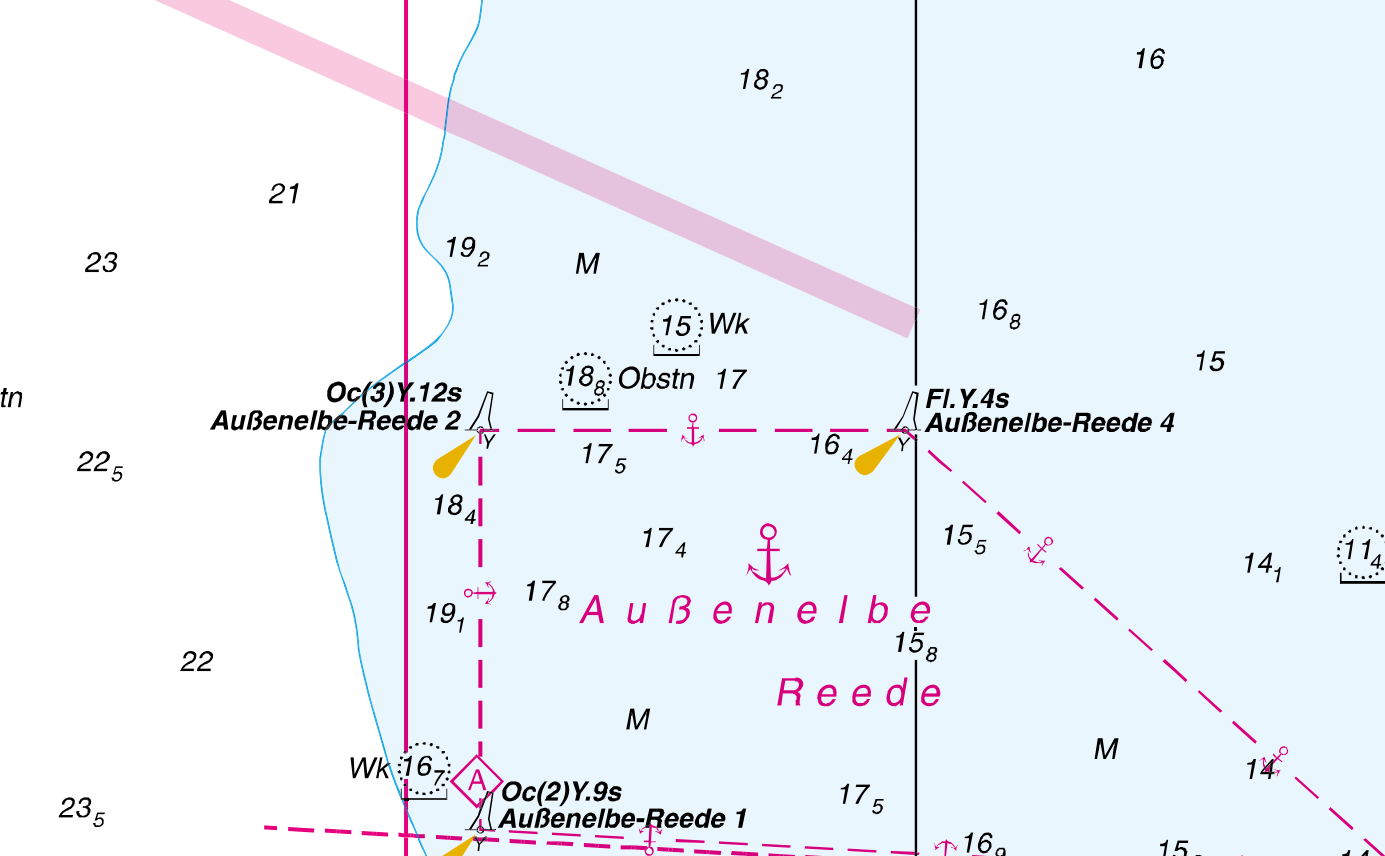
\includegraphics[width=0.8\linewidth]{glyphen}
					\caption[Beispiel eines Glyphs auf Basis einer Seekarte]{Auf diesem Seekartenausschnitt ist zu sehen, wie die Tonnen Außenelbe-Reede 2 und 4 durch Glyphen dargestellt werden, die viele Informationen transportieren. Bei ersterer ist \bspw die Information enthalten, dass es sich um eine gelbe einfarbige Tonne ohne Toppzeichen mit unterbrochenem Feuer in dreier-Gruppen in Gelb und einer Wiederkehr von \SI{12}{\second} handelt.}
					\label{fig:glyph}
				\end{figure}
			% end
		% end

		\subsection{Bildunterschriften}
			Eine \emph{Bildunterschrift} sollte immer eine kurze Interpretation/Einordnung des Bildes mit Verweisen auf die Abbildung enthalten. Dabei sollten das Bild und die Unterschrift idealerweise auch ohne den Haupttext verständlich sein, da die Abbildungen häufig als erstes angeschaut werden. Im Haupttext sollte nachher auf die Abbildung verwiesen, diese aber nicht beschrieben werden (die Beschreibung gehört in die Bildunterschrift). Ebenfalls sollte die zentrale Aussage der Grafik im Text wiedergefunden werden.
		% end
	% end

	\section{Wahrnehmung, Position und Layout}
		\label{sec:wahrnehmung}

		In diesem Abschnitt werden die elementaren visuellen Aufgaben sowie die Wahrnehmung verschiedener Channels behandelt. Daraus werden abschließend Begründungen für oder gegen bestimmte Designentscheidungen abgeleitet.

		\subsection{Wahrnehmungsmodelle von Ware}
			Das visuelle System des Menschen ist in mehrere Schichten geteilt (V1 bis V5), die unterschiedliche Aufgaben erfüllen, wobei die zu erfüllenden Aufgaben mit steigender Schicht komplexer und abstrakter werden. Die Schichten sind dabei in beide Richtungen verbunden und die Funktion und Interaktion zwischen den Schichten ist ein offenes Forschungsthema. Diese Idee der Schichten wurde von Colin Ware zu dem \emph{Wahrnehmungsmodell (von Ware)} zusammengefasst, welches die ablaufenden Prozesse in drei Gruppen/Stufen einteilt:
			\begin{enumerate}
				\item Parallele Verarbeitung elementarer visueller Merkmale statt. Diese Verarbeitung ist dabei nicht erlernbar und bei allen Menschen zum Großteil gleich.
				\item Mustererkennung; langsame und serielle Verarbeitung, welche trainierbar ist, sodass weniger Aufmerksamkeit benötigt wird.
				\item Sequentielle und zielgerichtete Verarbeitung; sehr langsame, aufmerksam gesteuerte, Übersetzung visueller Objekte in Sprache und anders herum.
			\end{enumerate}
			Die Kommunikation zwischen den Stufen verläuft dabei ebenfalls in beide Richtungen. Da die Wahrnehmung des gleichen Bildes nicht zu jedem Zeitpunkt und jedem Menschen das gleiche Ergebnis liefert, \dh die Verarbeitung ist nicht streng deterministisch, gibt es keine absolut "richtigen" und "falschen" Design für bestimmte Menschen. Eine solche Unterscheidung kann nur auf Basis gut verstandener, bei allen Menschen "gleichen", Prozesses erfolgen, \dh auf dem Stufe-1-System. Für eine bestimmte Menschengruppe kann eventuell auch auf Stufe 2 gewechselt werden, auf der auch bestimmte Mustererkennungen trainiert werden können.

			\subsubsection{Farbe und Farbmodelle}
				\label{subsubsec:farbe}

				Ein weiterer Aspekt der Wahrnehmung ist die Farbe, die durch drei (fast) unabhängige Größen definiert wird. Je nach Farbmodell sind dies \bspw der Rot-, Grün- und Blau-Anteil (RGB-Modell) oder Farbton, Helligkeit und Sättigung (HSV\footnote{Hue, Saturation und Value}-Modell).

				Das RGB-Modell ist dabei technisch vor allem deshalb relevant, da es einen engen Bezug zu den Rezeptoren auf der Netzhaut aufweist: Die drei Farbrezeptoren auf der Netzhaut sind S-, M- und L-Zapfen, die in der Reihenfolge kurze, mittlere und lange Wellenlängen detektieren (und damit blau, grün und grün-gelb erkennen). Andere Farben entstehen anschließend durch Mischung der Rezeptoren im Gehirn. Durch eine Kombination aller Rezeptoren wird rein die Helligkeit wahrgenommen, weshalb diese auch als unabhängiger Channel wahrgenommen wird.

				Ein weiteres Farbmodell ist das CIE-Farbmodell, welche die Gesamtheit der wahrnehmbaren und darstellbaren Farben erfasst. Dabei wurde bei der Gestaltung des Modells darauf geachtet, dass "Distanzen" im Farbraum wahrnehmungsgetreu modelliert werden. Dieses Farbmodell wird ebenfalls bei der Bewertung des Farbraums eines Monitors genutzt.
			% end

			\subsubsection{Farbskalen und Farbfehlsicht}
				In der Wahrnehmung und Visualisierung ist das HSV-Modell am relevantesten, da verschiedene Werte gut auf die Channels abgebildet werden können. Dabei werde innerhalb einer einzigen Visualisierung allerdings am besten immer nur ein Channel und maximal zwei verwendet. Dabei gibt es im Vergleich zu anderen Channels (abgesehen von der Position) die meisten Variationsmöglichkeiten. Dies ist gleichzeitig ein Vor- und ein Nachteil: Durch die starke Variation können sehr viele Daten abgebildet werden, allerdings sind die Skalen nicht unbedingt gut ablesbar. Durch Einschränkungen wie Farbfehlsicht werden die verfügbaren Farbskalen auf einige wenige eingegrenzt. Dabei werden drei Typen von Farbskalen unterschieden:
				\begin{itemize}
					\item \eqmakebox[colorMapping][l]{\emph{Kategorische Skala:}} unterschiedliche Farbtöne; konstante Helligkeit und Sättigung
					\item \eqmakebox[colorMapping][l]{\emph{Divergente Skala:}}   zwei unterschiedliche Farbtöne für zwei Hälften der Skala (\bspw positiv und negativ); Variation von Helligkeit und Sättigung; Mitte ist hell/weiß und markiert den Nullpunkt
					\item \eqmakebox[colorMapping][l]{\emph{Sequentielle Skala:}} konstanter Farbton, kein Gelb; monoton Helligkeits-/Sättigungsänderung
				\end{itemize}
				Dabei können die letzten beiden sowohl diskrete als auch kontinuierliche Daten abbilden. Bei dem Design einer Farbskala müssen verschiedene Einschränkungen wie Farbfehlsicht beachtet werden. Die üblichste Farbfehlsicht ist die Rot-Grün-Schwäche (Deuteranopie), weshalb diese Farben niemals gleichzeitig in einer Visualisierung genutzt werden sollten. Weitere Informationen zu Farbfehlsicht findet sich auf \href{https://en.wikipedia.org/wiki/Color_blindness}{Wikipedia}\footnote{\url{https://en.wikipedia.org/wiki/Color_blindness}}. Um die Nutzung von Farbskalen zu vereinfachen und bekannte Effekte einzubeziehen gibt es viele Tools, \bspw \href{https://colorbrewer2.org}{ColorBrewer}\footnote{\url{https://colorbrewer2.org/}} und \href{https://color.adobe.com/de/create/color-accessibility}{Adobe Color}\footnote{\url{https://color.adobe.com/de/create/color-accessibility}}.

				Als generelle Faustregel sollten sich die Enden der Skala immer von dem Hintergrund abheben, da diese meist am interessantesten sind. Bei einem dunklen Hintergrund sollten sie dementsprechend hell, bei einem dunklen Hintergrund (was aus unerfindlichen Gründen immer beliebter wird\dots) hell sein.
			% end
		% end

		\subsection{Elementare Visuelle Aufgaben}
			In diesem Abschnitt werden die elementaren visuellen Aufgaben behandelt, in die übergeordnete Aufgaben einsortiert werden können. Diese "high-level" Aufgaben ("Explain", "Explore" und "Enjoy") repräsentieren dabei die eigentliche Ziele, die viele elementare "low-level" Aufgaben enthalten können, die sich auf wirklich elementare Handlungen beziehen.

			Aus Anwender*innensicht muss ein Mensch immer die folgenden Schritte durchgehen, um eine Aufgabe abzuarbeiten: Die Informationen in der Visualisierung suchen, die Informationen aus der Visualisierung ablesen (auch \emph{Query} genannt) und die Informationen interpretieren (eventuell unabhängig von der Visualisierung). Dabei werden die Schritte üblicherweise nicht nur einmal, sondern mehrfach und nicht zwangsweise immer von Vorne bis Hinten durchlaufen. Dies ist in \autoref{fig:aufgabenVerarbeitung} dargestellt. Im Idealfall unterstützt eine Visualisierung alle drei Schritte, \dh die Aufgabe wird für den*die Nutzer*in in jedem Schritt vereinfacht\footnote{Ein Beispiel ist die Wahl der Farbskala: Durch die Wahl einer Skala in der nur die Helligkeit/Sättigung variiert wird, wird die Frage danach, ob etwas "mehr" oder "weniger" ist, intuitiver als bei einer "Regenbogen"-Skala.}. Es ist jedoch möglich, sich an schlechte Visualisierungen zu gewöhnen, \bzw diese zu lernen. Daher ist eine neue -- objektiv bessere -- Visualisierung eventuell weniger attraktiv, da das Design noch nicht vertraut ist.

			Innerhalb dieses einfachen dreischrittigen Prozesses können weiterhin die Schritte "Suchen" und "Query" in weitere Aufgaben eingeteilt werden, die in den nächsten beiden Abschnitten behandelt werden.

			\begin{figure}
				\centering
				\begin{tikzpicture}[->, cmp/.style = { draw, ellipse, minimum height = 1cm, minimum width = 2.8cm }, stp/.style = { draw, rectangle, minimum height = 0.75cm, minimum width = 2.8cm }]
					\node [stp] (search) {Suche};
					\node [stp, below = 1 of search] (query) {Query};
					\node [stp, below = 1 of query] (int) {Interpretation};

					\draw (search) to coordinate(a) (query);
					\draw (query) to coordinate(b) (int);
					\draw [dashed] (query.east) to[out = 45, in = -45] (search.east);
					\draw [dashed] (int.east) to[out = 45, in = -45] (query.east);
					\coordinate [above = 0.75 of search] (A);
					\coordinate [below = 0.75 of int] (B);

					\node [cmp, left = 3 of a] (task) {Aufgabe};
					\node [cmp, left = 3 of b] (human) {Mensch};

					\draw [dashed] (int) to (B) -| (human) to (task) |- (A) to (search);
				\end{tikzpicture}
				\caption{Aufgabenverarbeitungsprozess}
				\label{fig:aufgabenVerarbeitung}
			\end{figure}

			\paragraph{Beispiel}
				\todo{Elementare Visuelle Aufgaben: Beispiel; 3.35, 3.36, 3.37, 3.38, 3.39, 3.40, 3.41}
			% end

			\subsubsection{Suche}
				Die Suche kann innerhalb einer Matrix in vier Typen eingeteilt werden, siehe \autoref{tab:suche}: \emph{Look-Up}, \emph{Browsen}, \emph{Lokalisieren} und \emph{Explorieren}. Dabei sind alle Szenarien elementar und die Ausführung ist kurz (innerhalb einer Minute), dennoch benötigen die Aufgaben aufsteigend mehr Zeit. Dabei hängt sich die Unterscheidung nicht nur von der Aufgabe selbst, sondern auch von dem*der Anwender*in ab, \dh von Wissen über die Inhalte der Visualisierung und der Vertrautheit mit den genutzten räumlichen Strukturen\footnote{So ist das Ablesen der Einwohnerzahl von Berlin auf einer Weltkarte für die meisten Leser*innen vermutlich eher ein Look-Up, während das Ablesen der Einwohnerzahl von Marseille eher unter "Browsen" gefasst wird.}. Durch die wenigen bekannten Informationen ist "Explore" das anspruchsvollste Szenario.

				\begin{table}
					\centering
					\begin{tabular}{c|cc}
						\toprule
						                                                        & \textbf{Es ist bekannt, wonach gesucht wird.} & \textbf{Es sind höchstens Eigenschaft bekannt, nach denen gesucht wird.} \\ \midrule
						\textbf{Es ist bekannt, wo etwas gefunden werden kann.} &                \emph{Look-Up}                 &                              \emph{Browsen}                              \\
						\textbf{Es ist nicht bekannt, wo gesucht werden muss.}  &              \emph{Lokalisieren}              &                            \emph{Explorieren}                            \\ \bottomrule
					\end{tabular}
					\caption{Elementare Suchszenarien}
					\label{tab:suche}
				\end{table}

				\paragraph{Beispiel}
					\todo{Elementare Visuelle Aufgaben: Suche: Beispiel; 3.46, 3.48}
				% end
			% end

			\subsubsection{Query}
				Ein Query, \dh das Ablesen von Informationen aus einer Visualisierung, kann in sie Szenarien
				\begin{itemize}
					\item \eqmakebox[query][l]{\emph{Identifizieren:}} Suche von einer Eigenschaft genau eines Items
					\item \eqmakebox[query][l]{\emph{Vergleichen:}}    Suche von Unterschieden zwischen mehreren Items
					\item \eqmakebox[query][l]{\emph{Zusammenfassen:}} Suche von allen Items mit ähnlichen Eigenschaften
				\end{itemize}
				aufgeteilt werden. Dabei ist zusätzlich die Frage zu beantworten, was identifiziert/verglichen/zusammengefasst werden soll. Dies können beispielsweise einzelne Werte oder ganze "Muster" (insbesondere in Visual Analytics) sein.

				\paragraph{Beispiel}
					\todo{Elementare Visuelle Aufgaben: Query: Beispiel; 3.51, 3.52}
				% end
			% end

			\subsubsection{Einfluss der Abbildungskomponenten}
				Die einzelnen Komponenten einer Abbildung werden für verschiedenen Aufgaben primär verwendet: zur Interpretation werden Titel, Quelle, Legende, Achsenbeschriftungen sowie die Bildunterschrift (!) verwendet. Dahingegen fokussiert sich die Suche hauptsächlich auf den Grafikkörper, während beim Query zusätzlich die Legende sowie die Achsenwerte betrachtet werden.s
			% end
		% end

		\subsection{Eigenschaften Verschiedener Visueller Channels}
			In diesem Abschnitt werden die verschiedenen in \autoref{subsubsec:channels} eingeführten visuellen Channels den im vorherigen Abschnitt eingeführten Such- und Queryszenarien zugeordnet \bzgl ihrer Anwendbarkeit. Die Ergebnisse davon sind in \autoref{tab:channelsAufgaben} zusammengefasst.

			\paragraph{Auswahl/Hervorhebung}
				Um eine Element zu finden, also zu Lokalisieren und eventuell Identifizieren, eigen sich besonders \emph{selektive} Channels. Dabei werden die Markierungen mit einer einzigartigen Ausprägung ohne Suchen gefunden. Ebenfalls stellt sich heraus, dass die meisten wichtigen Channels (mit Ausnahmen bei der Form) selektiv sind. Allerdings ist die Wahrnehmung stark abhängig vom Kontrast, \dh den Eigenschaften der umliegend Items. Außerdem ist ein Channel, der zur Hervorhebung genutzt wird, nicht für andere Eigenschaften nutzbar und eine Nutzung mehrerer Channels zur Hervorhebung verschiedener Markierungen ist nicht sinnvoll.
			% end

			\paragraph{Ordnung}
				Um eine Ordnung zu Visualisieren, also zu Suchen und qualitativen Vergleichen, eignen sich \emph{ordinale} Channels für ordinale Datenvariablen. Dabei müssen die Ausprägungen der Channels eine natürliche, intuitive, Ordnung aufweisen (\zB groß/mittel/klein) und für einen Vergleich sollte keine Legende zu Rate gezogen werden müssen. Zwei Sonderfälle sind die Position, die nicht nur dem Vergleich, sondern auch der Strukturierung der Daten dient und damit jede Suche -- unabhängig von dem Query -- erleichtert. Außerdem kann die Orientierung sowohl für zyklische auch als linear Ordnungen genutzt werden (vgl.~"Uhr" und "Tacho").
			% end

			\paragraph{Differenzen}
				Zum Vergleich von Differenzen, \dh quantitativen Vergleichen, helfen \emph{quantitative} Channels. Die einzigen Channels, die dies verlässlich abbilden, sind Länge und Position unter der Voraussetzung, dass beide Skalen den Nullpunkt beinhalten und linear sind. Die menschlichen Reize und deren Verhältnis zu der objektiven Reizänderung werden dabei durch \emph{Stephens Power Law} beschrieben: Beispielsweise wird eine Sirene (\SI{120}{\deci\bel}) nicht \num{1000000}-mal lauter wahrgenommen als ein Gespräch (\SI{60}{\deci\bel}), obwohl sie entsprechend viel energiereicher ist. Dies wird durch den Exponent \(\alpha\) charakterisiert, welcher ausschließlich für die Länge \(\alpha = 1\) ist.
			% end

			\paragraph{Zusammenfassen}
				Zur Zusammenfassung von Daten, also zum Browsing/Exploring und Zusammenfassen, eigen sich \emph{assoziative} Channels sehr gut, da sie helfen, ähnliche Items als Gruppe wahrzunehmen. Bei "Explain"-Aufgaben kann die Ähnlichkeit dabei durch eine Abbildung auf kategorische Variablen vorgegeben werden, bei "Explore"/"Enjoy" kann die Ähnlichkeit auch eine kombinierte Wahrnehmung von Mustern in verschiedenen Channels sein. Dabei kann die Wahrnehmung verschiedener Muster allerdings kollidieren, was bei optischen Täuschungen ausgenutzt wird.
			% end
		% end

		\subsection{(Ungewollte) Einflüsse}
			In diesem Abschnitt werden einige (oft ungewollte) gegenseitige Einflüsse von verschiedenen Channels aufeinander behandelt. Diese räumlich beieinander liegen, damit die Wahrnehmung weniger beeinflusst wird. Dabei ist die Wahrnehmung fast immer von dem Verhältnis von Kontrast und Entfernung abhängig -- und vom Kontext.

			\paragraph{Kontrast, Perzeptuelle Länge und Farbnamen}
				Die \emph{perzeptuelle Länge} beschreibt dabei die Anzahl unterscheidbarer Werte je Channel, auch wenn die Unterscheidung erschwert wird. Üblicherweise sind das nicht viele, was insbesondere bei der Visualisierung verschiedener Kategorien relevant ist. Im Allgemeinen sind solche Farben und Formen unterscheidbar, die man benennen kann. Es sollten aber eigentlich nicht die Farben, sondern die Kategorien unterschieden werden. Um dies nicht zu erschweren, sollten so wenig Farben und Formen wie möglich verwendet werden.
			% end

			\paragraph{Gesichter, Bewegung und 3D aus Bildern}
				Da Menschen sehr gut darin sind/sein müssen, Gesichter schnell zu erkennen, neigen sie dazu, diese überall zu erkennen, was Darstellungsschwierigkeiten hervorrufen kann. Die zweit-wichtigste natürliche Aufgabe des Sehsinns ist die Erkennung von Bewegung und 3D-Grafiken auch aus "flachen" Bildern. Dies lässt sich nicht abschalten und beeinflusst die Wahrnehmung aller Channels.
			% end

			\subsubsection{Separierende und Integrierende Channels}
				Werden verschiedene visuelle Channels gleichzeitig eingesetzt, so ist zwischen \emph{separierende} und \emph{integrierenden} Channels zu unterscheiden: Bleibt von den einzelnen Variablen etwas übrig (\emph{separierend}) oder entsteht ein neuer Sinneseindruck (\emph{integrierend})? Beispielsweise ist Position und Form ein separierendes Paar, wohingegen der Rot- und Blau-Kanal einer Farbe integrierend sind. Je nach Anwendung ist beides sinnvoll, da separierende Paare mehr Datenvariablen, integrierende Paare hingegen mehr unterscheidbare Werte, erlauben. Dabei ist, wie so oft, der Übergang zwischen den Kategorien fließend und abhängig vom konkreten Anwendungsfall. Eine kleine Übersicht ist in \autoref{fig:separierendIntegrierend} gegeben.

				\begin{figure}
					\centering
					\begin{tikzpicture}[b/.style = { draw, rectangle, minimum height = 0.75cm, minimum width = 2cm }]
						\node [b] (a) {Farbton};
						\node [b, right = 1 of a] (b) {Farbton};
						\draw (a) to coordinate(A) (b);
						\node [b, below = 0.1 of a] (a) {Helligkeit};
						\node [b, right = 1 of a] (b) {Farbe};
						\draw (a) to (b);
						\node [b, below = 0.1 of a] (a) {Höhe};
						\node [b, right = 1 of a] (b) {Breite};
						\draw (a) to (b);
						\node [b, below = 0.1 of a] (a) {Form};
						\node [b, right = 1 of a] (b) {Größe};
						\draw (a) to (b);
						\node [b, below = 0.1 of a] (a) {Farbton};
						\node [b, right = 1 of a] (b) {Größe};
						\draw (a) to (b);
						\node [b, below = 0.1 of a] (a) {Farbton};
						\node [b, right = 1 of a] (b) {Form};
						\draw (a) to (b);
						\node [b, below = 0.1 of a] (a) {Farbton};
						\node [b, right = 1 of a] (b) {Bewegung};
						\draw (a) to (b);
						\node [b, below = 0.1 of a] (a) {Position};
						\node [b, right = 1 of a] (b) {\dots};
						\draw (a) to coordinate(B) (b);

						\node [above = 0.75/2+0.1 of A] {\textbf{Integrierend}};
						\node [below = 0.75/2+0.1 of B] {\textbf{Separierend}};
					\end{tikzpicture}
					\caption{Vergleich separierender und integrierender Channels}
					\label{fig:separierendIntegrierend}
				\end{figure}
			% end
		% end

		\subsection{Position, Layout und Komposition: Suchen vs. Finden}
			Die zentrale Idee von geschicktem Layouting ist, die Suche zu erleichtern oder zu umgehen (von "Suchen" zu "Finden"). Ein Beispiel ist die Anordnung von einzelnen Diagrammen so zu gestalten, dass ähnliche räumliche Strukturen nebeneinander liegen (\zB gemeinsame y-Achsen). Dadurch kann eine einmal "gelesene" Struktur auf die benachbarten Visualisierungen angewendet und zeitsparend genutzt werden.

			\subsubsection{Beispiele}
				\todo{Position, Layout und Komposition: Beispiele; 3.87, 3.88, 3.89, 3.90, 3.91}
			% end

			\subsubsection{Zusammengesetzte Visualisierungen}
				Zusammengesetzte Visualisierungen können genutzt werden, um komplexe Daten abzubilden. Dabei gibt es verschiedene Varianten bis hin zu interagierenden Visualisierungen (siehe \autoref{fig:zusammengesetzteVisualisierungen}). Dabei gibt es einige visuelle Designmuster, \zB:
				\begin{itemize}
					\item \eqmakebox[zusmVis][l]{\emph{Juxtaposition (Gegenüberstellung):}} häufigstes Designmuster; die View stehen nebeneinander, die Verbindung ist implizit (\zB durch eine gemeinsame Achse)
					\item \eqmakebox[zusmVis][l]{\emph{Superimposition (Überlagerung):}} zwei Views nutzen den gleichen Raum, dadurch wird ein räumlicher Bezug hergestellt; gemeinsame Achse oder Markierungen
					\item \eqmakebox[zusmVis][l]{\emph{Overloading (Überladung):}} eine Visualisierung wird ergänzend in der Hauptvisualisierung dargestellt; Nutzung der gleichen visuellen Abbildung auf die Position, aber \ggf andere Marks/Channels
					\item \eqmakebox[zusmVis][l]{\emph{Nesting (Einbettung):}} Marks sind selbst (kleine) Visualisierungen; stellt einen Bezug zwischen "Überblick" und "Detail" her
				\end{itemize}

				\begin{figure}
					\centering
					\begin{tikzpicture}[->, every node/.style = { draw, rectangle, minimum height = 0.7cm, minimum width = 4.5cm }]
						\node [label = above:{bestimmte Aufgabe}] (a) {Einzelne Vis.};
						\node [right = 2 of a, label = above:{verschiedene Perspektiven}] (b) {Zusammengesetzte Vis.};
						\node [below = 1 of a, label = below:{Freiheitsgrade für Nutzer*innen}] (c) {Interaktive Vis.};
						\node [right = 2 of c, label = below:{komplexe Aufgaben}] (d) {Interagierende Vis.};

						\draw (a) to (b);
						\draw (a) to (c);
						\draw (b) to (d);
						\draw (c) to (d);
					\end{tikzpicture}
					\caption{Verschiedene Arten von zusammengesetzten Visualisierungen}
					\label{fig:zusammengesetzteVisualisierungen}
				\end{figure}

				\paragraph{Beispiele}
					\todo{Position, Layout und Komposition: Zusammengesetzte Visualisierungen: Beispiele; 3.97, 3.98, 3.99, 3.100}
				% end
			% end
		% end
	% end

	\section{Interaktion} % 5.1, 5.3, 5.4, 5.5, 5.6, 5.7, 5.8, 5.20, 5.21, 5.68
		\label{sec:interaktion}

		\todo{Content}

		\subsection{Benutzungsschnittstellen} % 5.9, 5.10, 5.11, 5.12, 5.13, 5.17, 5.30
			\todo{Content}

			\subsubsection{Bedienung und Interaktion nach Norman} % 5.14, 5.15, 5.16
				\todo{Content}
			% end

			\subsubsection{ISO 9241} % 5.18
				\todo{Content}
			% end

			\subsubsection{Interaktionsmodi nach Spence} % 5.22, 5.23
				\todo{Content}

				\paragraph{Kontinuierliche Interaktion} % 5.24
					\todo{Content}
				% end

				\paragraph{Schrittweise Interaktion} % 5.25, 5.26, 5.27
					\todo{Content}
				% end

				\paragraph{Passive Interaktion} % 5.28
					\todo{Content}
				% end

				\paragraph{Gemischte Interaktion} % 5.29
					\todo{Content}
				% end
			% end
		% end

		\subsection{Interaktionstechniken} % 5.31, 5.32, 5.33, 5.48
			\todo{Content}

			\subsubsection{Systemnahe Interaktionstechniken} % 5.35
				\todo{Content}

				\paragraph{Selektion} % 5.36
					\todo{Content}
				% end

				\paragraph{Navigation} % 5.37, 5.38, 5.39
					\todo{Content}
				% end

				\paragraph{Shneidermans Mantra} % 5.40, 5.41, 5.42, 5.43
					\todo{Content}
				% end

				\paragraph{Fokus und Kontext} % 5.44, 5.45
					\todo{Content}
				% end

				\paragraph{Überblick und Detail} % 5.46
					\todo{Content}
				% end

				\paragraph{Brushing und Linking} % 5.47
					\todo{Content}
				% end
			% end

			\subsubsection{Kategorien der Interaktion nach Yi et al.} % 5.49, 5.50, 5.51, 5.52
				\todo{Content}
			% end
		% end

		\subsection{Design} % 5.54, 5.55
			\todo{Content}

			\subsubsection{Leitsätze} % 5.56
				\todo{Content}

				\paragraph{Navigation} % 5.57
					\todo{Content}
				% end

				\paragraph{Organisation} % 5.58
					\todo{Content}
				% end

				\paragraph{Erzeugung von Aufmerksamkeit} % 5.59
					\todo{Content}
				% end

				\paragraph{Unterstützung der Dateneingabe} % 5.60
					\todo{Content}
				% end
			% end

			\subsubsection{Prinzipien} % 5.61
				\todo{Content}

				\paragraph{Ermittlung des fachlichen Niveaus des Nutzers} % 5.62
					\todo{Content}
				% end

				\paragraph{Ermittlung der Arbeitsaufgaben} % 5.63
					\todo{Content}
				% end

				\paragraph{Wahl des Interaktionsstils} % 5.64
					\todo{Content}
				% end

				\paragraph{Die Acht Goldenden Regeln der Gestaltung} % 5.65, 5.66
					\todo{Content}
				% end
			% end

			\subsubsection{Menschliche Reaktionszeit} % 5.67
				\todo{Content}
			% end
		% end
	% end
% end

\chapter{Spezialisierte Visualisierungstechniken} % 6.3, 6.4, 6.5, 6.52
	\todo{Content}

	\section{Hochdimensionale Daten} % 6.6, 6.7, 6.8, 6.9, 6.10, 6.11, 6.17, 6.53
		\todo{Content}

		\subsection{Quantitative Daten} % 6.12
			\todo{Content}

			\subsubsection{Scatterplot-Matrix} % 6.14, 6.15, 6.16
				\todo{Content}
			% end

			\subsubsection{Starplot} % 6.18, 6.19, 6.20, 6.23
				\todo{Content}

				\paragraph{Small Multiple Plots} % 6.21, 6.22
					\todo{Content}
				% end
			% end

			\subsubsection{Parallele Koordinaten} % 6.24, 6.25, 6.26, 6.27
				\todo{Content}

				\paragraph{\dots mit Interaktion} % 6.28
					\todo{Content}
				% end
			% end

			\subsubsection{RadViz} % 6.29, 6.30, 6.31
				\todo{Content}
			% end
		% end

		\subsection{Kategorische Daten} % 6.32
			\todo{Content}

			\subsubsection{Parallel Sets} % 6.34, 6.35, 6.36, 6.37
				\todo{Content}

				\paragraph{\dots mit Interaktion} % 6.38
					\todo{Content}
				% end
			% end

			\subsubsection{Mosaic-Plot} % 6.39, 6.40, 6.41
				\todo{Content}
			% end

			\subsubsection{KV-Map} % 6.42, 6.43, 6.44, 6.45, 6.45, 6.46, 6.47, 6.48
				\todo{Content}
			% end

			\subsubsection{Tabelle} % 6.49, 6.50, 6.51
				\todo{Content}
			% end
		% end
	% end

	\section{Große Datenmengen} % 6.54, 6.55
		\todo{Content}

		\subsection{Ordnen} % 6.57, 6.57
			\todo{Content}

			\subsubsection{Dimensionsreduktion und Feature Selektion} % 6.59, 6.60, 6.61, 6.62, 6.63, 6.82
				\todo{Content}

				\paragraph{Principal Component Analysis (PCA)} % 6.64, 6.65, 6.66, 6.67
					\todo{Content}
				% end

				\paragraph{Linear Discriminant Analysis (LDA)} % 6.68, 6.69
					\todo{Content}
				% end

				\paragraph{Multidimensional Scaling (MDS)} % 7.70, 6.71, 6.72, 6.73
					\todo{Content}
				% end

				\paragraph{Self-Organizing Map (SOM)} % 6.74, 6.75, 6.76, 6.77, 6.78, 6.79, 6.80, 6.81
					\todo{Content}
				% end
			% end
		% end

		\subsection{Aggregieren} % 6.83, 6.84, 6.85, 6.86, 6.87, 6.88, 6.89, 6.90
			\todo{Content}
		% end
	% end

	\section{Zeitbasierte Daten} % 7.3, 7.4, 7.5, 7.6, 7.29
		\label{sec:visZeitbasiert}

		\todo{Content}

		\subsection{Viele Zeitreihen} % N/A
			\todo{Content}

			\subsubsection{Filtern} % 7.7
				\todo{Content}
			% end

			\subsubsection{Heatmaps} % 7.8
				\todo{Content}

				\paragraph{\dots mit Aggregation} % 7.12
					\todo{Content}
				% end
			% end

			\subsubsection{Horizon Plots} % 7.9, 7.10, 7.11
				\todo{Content}
			% end

			\subsubsection{Small Multiples} % 7.13
				\todo{Content}

				\paragraph{\dots mit Aggregation} % 7.14
					\todo{Content}
				% end
			% end
		% end

		\subsection{Periodische Zeitreihen} % 7.15
			\todo{Content}

			\subsubsection{Spiral Layouts} % 7.16, 7.17
				\todo{Content}
			% end

			\subsubsection{Matrix-Layout} % 7.18
				\todo{Content}
			% end
		% end

		\subsection{Diskrete Ereignisse} % 7.19, 7.20, 7.21
			\todo{Content}

			\subsubsection{Sequenzbaum} % 7.22, 7.23, 7.24, 7.25, 7.26, 7.27
				\todo{Content}
			% end
		% end
	% end

	\section{Graphen und Bäume} % 7.30, 7.31, 7.32, 7.33, 7.34, 7.65
		\label{sec:visGraphen}

		\todo{Content}

		\subsection{Bäume} % 7.35, 7.47
			\todo{Content}

			\subsubsection{Node-Link-Diagramm} % 7.36, 7.37, 7.38
				\todo{Content}
			% end

			\subsubsection{Radiales Layout} % 7.39
				\todo{Content}
			% end

			\subsubsection{TreeMaps} % 7.40, 7.41
				\todo{Content}

				\paragraph{Cushions} % 7.42
					\todo{Content}
				% end

				\paragraph{Squarified} % 7.43, 7.44
					\todo{Content}
				% end
			% end

			\subsubsection{Icicle Plot und Sunburst} % 7.45, 7.46
				\todo{Content}
			% end
		% end

		\subsection{Allgemeine Graphen} % 7.48, 7.49, 7.50
			\todo{Content}

			\subsubsection{Layouts} % 7.51
				\todo{Content}

				\paragraph{Force-Directed} % 7.52, 7.53, 7.54
					\todo{Content}
				% end

				\paragraph{Layer-Based: Sugiyama} % 7.55, 7.56, 7.57
					\todo{Content}
				% end

				\paragraph{Constraint-Based: Metro-Map} % 7.58, 7.59, 7.60
					\todo{Content}
				% end
			% end

			\subsubsection{(Hierarchisches) Edge-Bundling} % 7.61, 7.62
				\todo{Content}
			% end
		% end

		\subsection{"Search, Show Context, Expand on Demand"} % 7.63, 7.64
			\todo{Content}
		% end
	% end

	\section{Geobasierte Daten und Karten} % 8.1, 8.4, 8.5, 8.6, 8.7, 8.8, 8.9, 8.10, 8.11, 8.12, 8.90
		\label{sec:karten}

		\todo{Content}

		\subsection{Karten als Metapher} % 8.13, 8.14, 8.15, 8.16, 8.17, 8.18, 8.19, 8.24, 8.25, 8.55, 8.56
			\todo{Content}

			\subsubsection{Karten und Schematisierungen} % 8.20, 8.21, 8.22, 8.23
				\todo{Content}
			% end
		% end

		\subsection{Geobezogene Daten} % 8.26, 8.27, 8.28, 8.29
			\todo{Content}

			\subsubsection{Kartenprojektion} % 8.30, 8.31, 8.32, 8.35, 8.36, 8.37, 8.38
				\todo{Content}

				\paragraph{Plattkarte} % 8.32
					\todo{Content}
				% end

				\paragraph{Mercator Projektion} % 8.33
					\todo{Content}
				% end

				\paragraph{Winkel-Tripel} % 8.34
					\todo{Content}
				% end
			% end

			\subsubsection{Verzerrte Darstellungen} % 8.39, 8.40, 8.41, 8.42
				\todo{Content}

				\paragraph{Metro-Map} % 8.43
					\todo{Content}
				% end

				\paragraph{(Stetige) Kartogramme} % 8.44, 8.45, 8.46, 8.47, 8.48, 8.49, 8.50, 8.51
					\todo{Content}
				% end
			% end

			\subsubsection{Abstrakte Geovisualisierungen} % 8.52, 8.53, 8.54
				\todo{Content}
			% end
		% end

		\subsection{Nicht-Geobezogene Daten} % 8.57, 8.58, 8.59, 8.60, 8.61, 8.69
			\todo{Content}

			\subsubsection{Wikipedia World Map} % 8.62, 8.63
				\todo{Content}

			\subsubsection{Themescapes} % 8.64
				\todo{Content}
			% end

			\subsubsection{Themengebiete} % 8.65
				\todo{Content}
			% end

			\subsubsection{Gmap World of Music} % 8.66
				\todo{Content}
			% end

			\subsubsection{Metro-Map Immitation} % 8.67
				\todo{Content}
			% end

			\subsubsection{Rekonstruktion von Terrain aus Knotenattribut} % 8.68
				\todo{Content}
			% end
		% end

		\subsection{Raum-Zeit Daten} % 8.84, 8.85, 8.86
			\todo{Content}

			\subsubsection{Darstellung von Richtungen} % 8.87
				\todo{Content}
			% end

			\subsubsection{Darstellung von Geschwindigkeiten} % 8.88
				\todo{Content}
			% end

			\subsubsection{Darstellung von Vielen Trajektorien} % 8.89
				\todo{Content}
			% end
		% end
	% end
% end
